% Layout starter only: replace every example node and edge from an evidence ledger.
% Relative placement uses rendered node heights, including wrapped mathematics.
\documentclass[border=8mm]{standalone}
\usepackage{fontspec,amsmath,unicode-math,tikz}
\usetikzlibrary{arrows.meta,positioning,fit,calc}
\setmainfont{TeX Gyre Termes}
\setmathfont{TeX Gyre Termes Math}
\definecolor{ink}{HTML}{203548}
\definecolor{blue}{HTML}{326C91}
\definecolor{green}{HTML}{397D69}
\definecolor{purple}{HTML}{755991}
\tikzset{
  box/.style={draw=ink!60,fill=white,rounded corners=1.5mm,
    text width=5.1cm,inner xsep=2mm,inner ysep=2mm,align=center,
    font=\fontsize{10.5}{12.5}\selectfont,text=ink},
  construction/.style={box,draw=blue,fill=blue!4},
  arithmetic/.style={box,draw=green,fill=green!4},
  analytic/.style={box,draw=purple,fill=purple!4},
  direct/.style={-{Stealth[length=2mm]},draw=ink,line width=.7pt,
    shorten <=1mm,shorten >=1mm},
  technical/.style={-{Stealth[length=1.8mm]},draw=gray,line width=.5pt,
    shorten <=1mm,shorten >=1mm}
}
\begin{document}
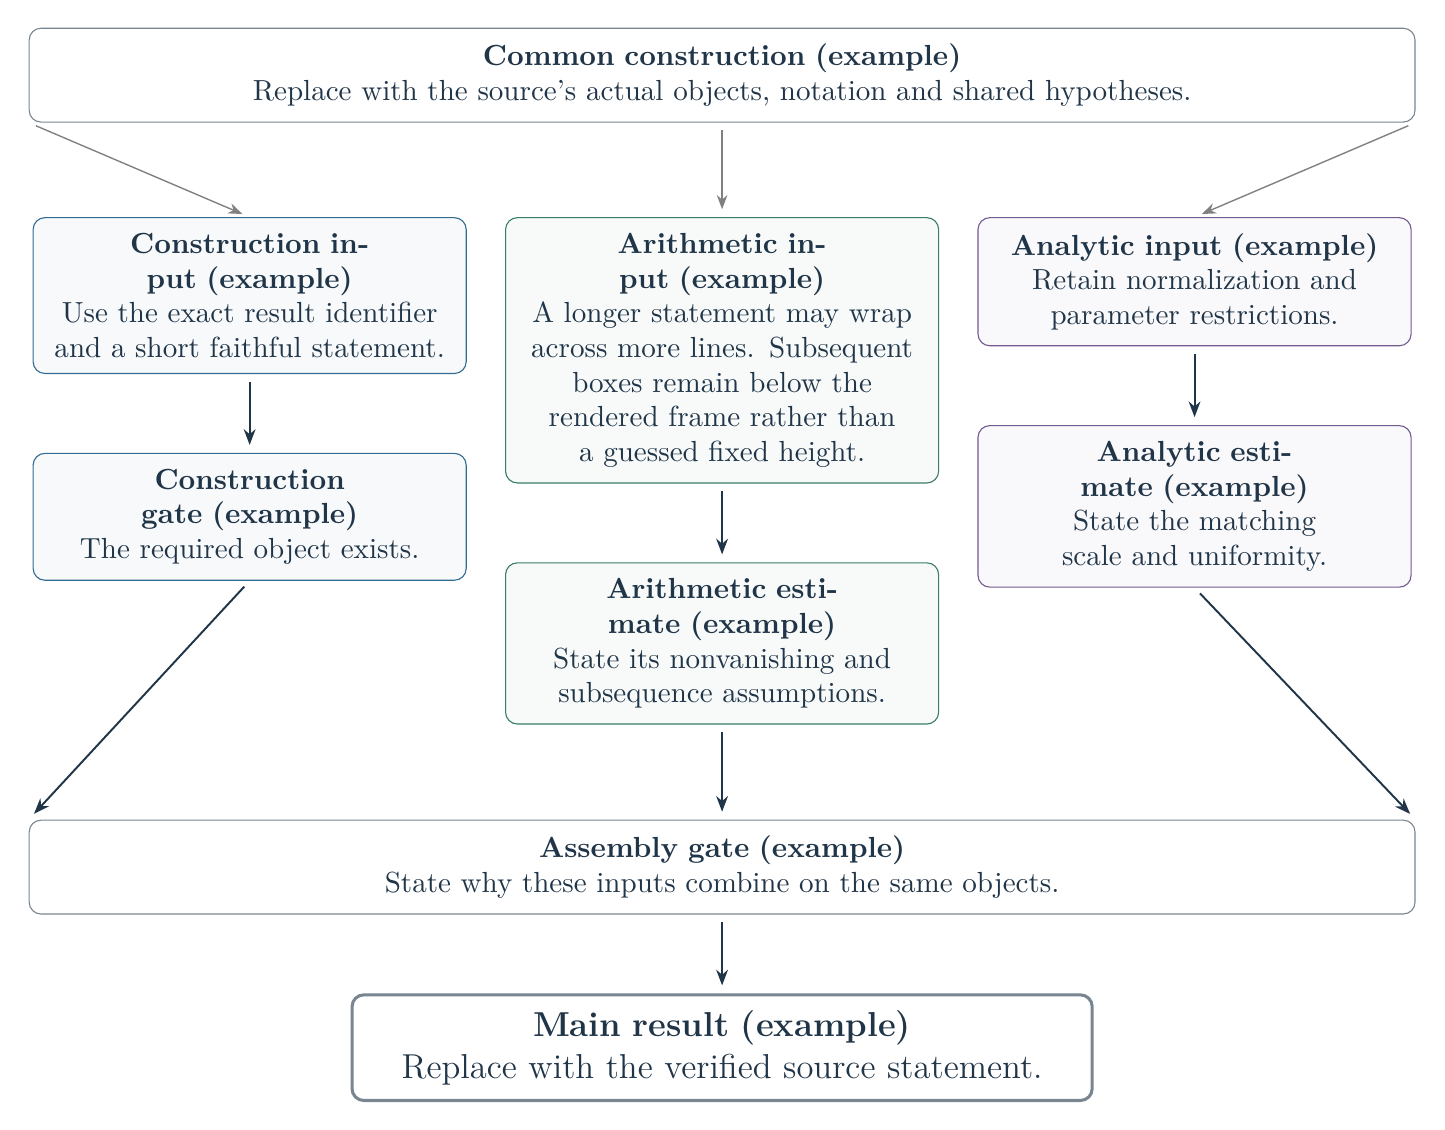
\begin{tikzpicture}[x=1cm,y=1cm]
  \node[box,text width=17.2cm] (setup)
    {\textbf{Common construction (example)}\\
     Replace with the source's actual objects, notation and shared hypotheses.};
  \node[construction,below=12mm of setup,xshift=-6cm] (a1)
    {\textbf{Construction input (example)}\\
     Use the exact result identifier and a short faithful statement.};
  \node[arithmetic,below=12mm of setup] (b1)
    {\textbf{Arithmetic input (example)}\\
     A longer statement may wrap across more lines. Subsequent boxes remain below
     the rendered frame rather than a guessed fixed height.};
  \node[analytic,below=12mm of setup,xshift=6cm] (c1)
    {\textbf{Analytic input (example)}\\
     Retain normalization and parameter restrictions.};
  \node[construction,below=10mm of a1] (a2)
    {\textbf{Construction gate (example)}\\The required object exists.};
  \node[arithmetic,below=10mm of b1] (b2)
    {\textbf{Arithmetic estimate (example)}\\State its nonvanishing and subsequence assumptions.};
  \node[analytic,below=10mm of c1] (c2)
    {\textbf{Analytic estimate (example)}\\State the matching scale and uniformity.};
  % The envelope includes the tallest/lower branch endpoint.
  \node[fit=(a2)(b2)(c2),inner sep=0pt] (branchrow) {};
  \node[box,text width=17.2cm,below=12mm of branchrow] (gate)
    {\textbf{Assembly gate (example)}\\State why these inputs combine on the same objects.};
  \node[box,text width=9cm,below=10mm of gate,line width=1.1pt,
    font=\fontsize{12.5}{15}\selectfont] (main)
    {\textbf{Main result (example)}\\Replace with the verified source statement.};
  \draw[technical] (setup.south west)--(a1.north);
  \draw[technical] (setup.south)--(b1.north);
  \draw[technical] (setup.south east)--(c1.north);
  \draw[direct] (a1.south)--(a2.north);
  \draw[direct] (b1.south)--(b2.north);
  \draw[direct] (c1.south)--(c2.north);
  \draw[direct] (a2.south)--(gate.north west);
  \draw[direct] (b2.south)--(gate.north);
  \draw[direct] (c2.south)--(gate.north east);
  \draw[direct] (gate.south)--(main.north);
\end{tikzpicture}
\end{document}
